\chapter{\label{chap:state}Bestehende Konzepte}
Sowohl integriert in Radwegen, als auch für den Einsatz in Kraftfahrzeugen gibt es bereits Projekte zu Ampelassistenten in Bordcomputern, Navigationssystemen, oder als mobile Applikation. Solche Anwendungen erkennen rote Ampeln und ermitteln die optimale Fahrgeschwindigkeit für die Grüne Welle. Auch Erweiterungen für Fahrräder werden immer vielfältiger --- vom einfachen Navigationssystem bis hin zu intelligenten Aufsätzen, die an das \gls{Smartphone} gekoppelt sind.
% ### Grüne Welle ###
\section{Ampelinformationssysteme}
Unter dem Prinzip "'Grüne Welle"' wird die Abstimmung der Ampelschaltzustände verstanden, sodass ein Fahrzeug in einer bestimmten Geschwindigkeit mehrere Ampeln passieren kann, ohne anhalten zu müssen. Im folgenden Abschnitt werden die existierenden Lösungen und Ansätze für Ampel- informationssysteme im Auto und für RadfahrerInnen dargestellt.
\subsection{Grüne Welle auf Radwegen}
In Kopenhagen unterstützen grüne \glspl{LED} auf Radwegen die RadfahrerInnen indem sie, wenn diese mit einem Tempo von 20 km/h fahren, sie begleiten und so signalisieren, dass sie sich auf der "'Grünen Welle"' befinden.\\
Abbildung \ref{fig:copenhagen} zeigt einen solchen Radweg mit einem Fahrradfahrer, der sich im "'grünen Bereich"' befindet. Zusätzlich erkennen Sensoren im Radweg Fahrradgruppen und veranlassen dann die Ampel zu einer längeren Grünphase. In einem anderen Stadtteil sind Leuchttafeln am Radwegrand installiert, die die verbleibende Zeit der Ampelphase anzeigen. \cite{KopIng}\\
Kopenhagen als Vorbild nehmend, hat Berlin mit vier Ampeln in Schöneberg eine Grüne Welle für RadfahrerInnen umgesetzt und plant bereits die zweite. \cite{BZ}\\ 
Auch hier möchte man die Benutzung des Rades attraktiver machen und den Fahrradverkehr beschleunigen.
\begin{figure}[H]  
    \centering  
    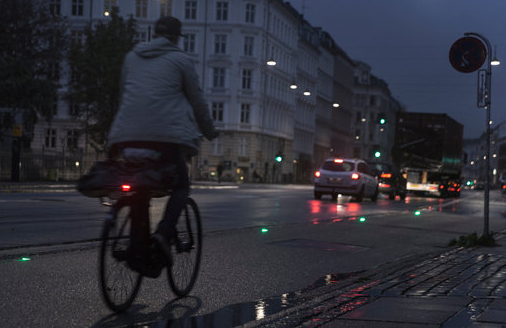
\includegraphics[width=0.6\textwidth]{copenhagen} 
    \grayRule
    \caption[Grüne Welle durch \glspl{LED}]{Kopenhagen: \glspl{LED} signalisieren die Grüne Welle bei 20 km/h  Quelle: \cite{NYT}}
     \label{fig:copenhagen}
\end{figure}
% ### AUTO ###
\subsection{Ampelinformationssysteme im Auto}
In den letzten Jahrzehnten gab es immer wieder Intentionen, eine Anzeige von Geschwindigkeitsempfehlungen im Fahrzeug umzusetzen. Der folgende Abschnitt stellt existierende Lösungen und Ansätze für Ampelinformationssysteme im Auto vor.
% ### WOLFSBURGER WELLE ###
\subsection*{Projekt Wolfsburger Welle}
Die VW-Forschung initiierte in den 80er Jahren mit dem Projekt "'Wolfsburger Welle"' die ersten Untersuchungen zu "'Grünen Welle"'-Informationen im Fahrzeug mit der Idee, beim Annähern an eine Ampel die optimale Geschwindigkeit im Fahrzeug vorzugeben.\cite{Welle} "Dazu sendet die Ampelanlage ihren aktuellen Phasenzustand und eine Prognose für den nächsten Zustandwechsel an alle Fahrzeuge, die sich annähern. Der Fahrzeugcomputer setzt dann die aktuelle Fahrzeuggeschwindigkeit mit dem Abstand zur Ampel und der aktuellen Ampelphase in Bezug. Daraus wird errechnet, ob das Fahrzeug im Moment mit der grünen Welle ’mitschwimmt’ oder ob die Geschwindigkeit außerhalb des optimalen Bereichs liegt". \cite{MenschMaschine}
%%% TRAVOLUTION %%%
\subsection*{\label{sec:travolution}Projekt Travolution}
Im Sommer 2008 wurde das Projekt \textsc{Travolution} (TRAffic \& eVOLUTION), von den Projektpartnern\footnote{\cite{Travolution}} abgeschlossen. Es besteht aus den Teilprojekten \textsc{verkehrsadaptive Netzsteuerung mit Genetischen Algorithmen} und \textsc{Der informierte Fahrer}. Im Netzsteuerungsprojekt wurden 46 \glspl{LSA} in Ingolstadt mit der Netzsteuerungssoftware \textsc{Balance} ausgestattet, wodurch sie intelligent auf den Verkehr reagieren und die Schaltung an den Verkehr anpassen.  Ziel des zweiten Teilprojektes war es, die Autofahrer über die Ampelphasen zu informieren. Die \gls{C2I} auf Basis von \gls{WLAN} umsetzend, senden mit Kommunikationsmodulen ausgestattete Ampeln die Grünphasen an den Bordcomputer der Autos, welcher dann die Geschwindigkeit für ein reibungsloses Passieren errechnet\cite{Stvtechnik} und wie in Abbildung \ref{fig:travolution} zu sehen ist, anzeigt. Im Rahmen des Projektes wurden zwei Anwendungsfälle umgesetzt. Die Restrotanzeige -- die die Dauer der verbleibenden Rotphase angibt, und die "'Dynamische Grüne Welle"' -- die Anzeige der \gls{Progressionsgeschwindigkeit}\footnote{ Geschwindigkeit die gehalten werden muss, um die Grüne Welle zu erreichen}.
Die Vorhersage der Schaltbilder ist aufgrund der verkehrsabhängigen Logik bei nicht festzeitgesteuerten \glspl{LSA} nur mit einer gewissen Wahrscheinlichkeit möglich. So werden sekündlich die Grünwahrscheinlichkeiten vom \gls{LSA}-Kommunikationsmodul aktualisiert und an das Fahrzeugmodul gesendet, welches diese in Relation zu eigener Position, Geschwindigkeit und Richtung setzt und die entsprechende Empfehlung ausgibt.\\
\begin{figure}[H]  
    \centering  
    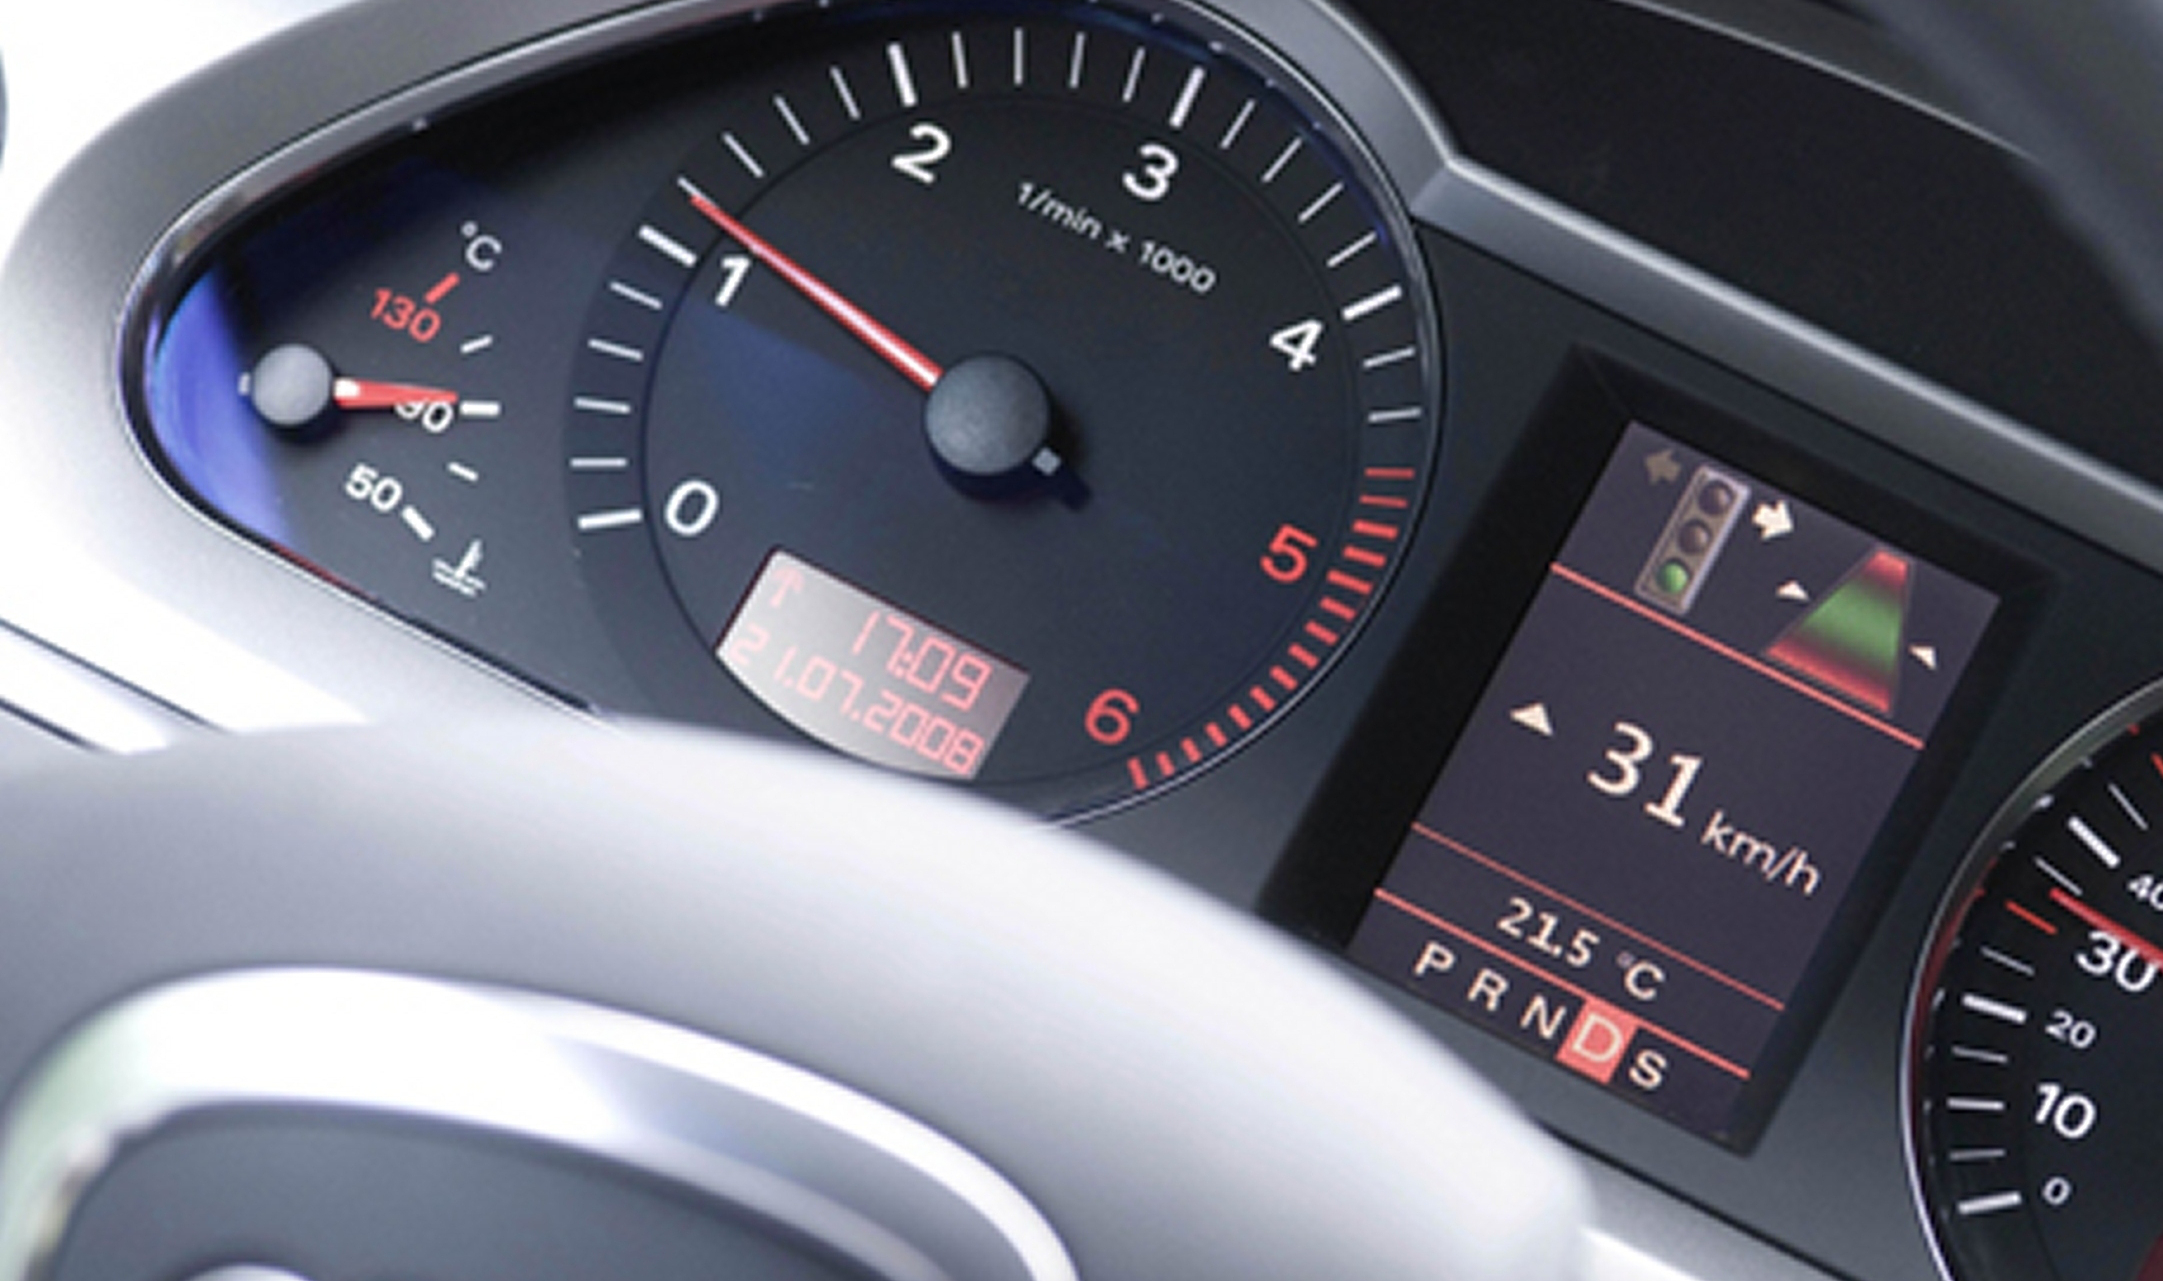
\includegraphics[width=0.7\textwidth]{travolution}   
    \grayRule
    \caption[Projekt Travolution]{Der Bordcomputer zeigt die optimale Geschwindigkeit an. Quelle: \cite{Travolution}}
    \label{fig:travolution}
\end{figure} 
Fundierend auf \textsc{Travolution} sind Folgeprojekte wie zum Beispiel das ebenfalls von Audi ins Leben gerufene "'Ampelinfo online"' entstanden. Über Mobilfunk ist in der \gls{C2X}-Anwendung das Auto mit dem zentralen Verkehrsrechner, welcher die Ampelanlagen steuert, vernetzt und visualisiert die entsprechenden Informationen im Bordcomputer. \cite{Ampelinfo}
%%% KOLIBRI %%%
\subsection*{\label{sec:kolibri}Projekt Kolibri}
In Bayern wurde im April 2011 das Pilot-Projekt \textsc{Kolibri}\footnote{ Kooperative Lichtsignaloptimierung -- Bayrisches Pilotprojekt} mit den Teststrecken der B13 bei München mit sieben und der St2145 in der Nähe von Regensburg mit acht ampelgeregelten Kreuzungen gestartet. Gemeinsam untersuchten die Projektpartner\footnote{ \url{http://www.kolibri-projekt.de/Sites/kolibri3.html}} die Funktionen und Auswirkungen eines Ampelassistenten außerhalb von Ortschaften. \cite{kolibri}\\ 
"'Per Mobilfunk übertragen die Ampeln ihre Daten an die Zentrale der TRANSVER GmbH. Dort wertet sie ein Computer aus und sendet die Ergebnisse an die Fahrzeuge. Ein Anzeigefeld im Bordcomputer oder eine Applikation auf dem \gls{Smartphone} zeigt an, ob sich das Fahrzeug in der Grünen Welle bewegt."' \cite{kolibriTUM}\\
Die FahrerInnen wurden sowohl fahrzeugintegriert\footnote{ On-Board-Computer} als auch via \gls{Smartphone}, wie Abbildung \ref{fig:kolibri} zeigt, über die Schaltung der nächsten Ampel informiert und erhielten Empfehlungen über die aktuelle \gls{Progressionsgeschwindigkeit}. Nach zwei Jahren erfolgreicher Arbeit war das Pilotprojekt abgeschlossen.\\
\begin{figure}[H]  
    \centering  
    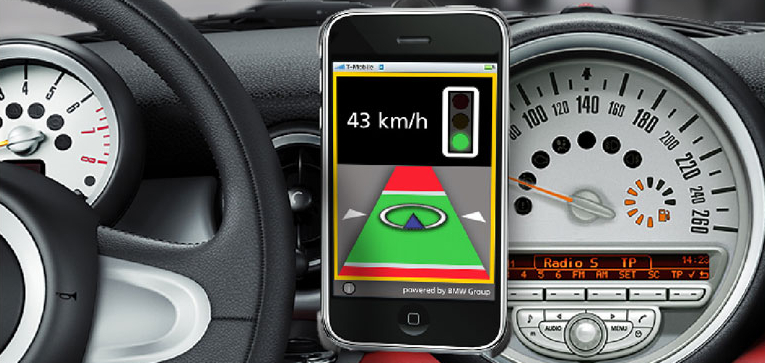
\includegraphics[width=0.7\textwidth]{kolibri}   
    \grayRule
    \caption[Projekt Kolibri]{Anzeige der Geschwindigkeitsempfehlung. Quelle: \cite{kolibri}}
    \label{fig:kolibri}
\end{figure} 
% TELEMATIK
\subsection*{Projekt Testfeld Telematik}
Ende des Jahres 2013 wurde in Wien das Projekt \textsc{Testfeld Telematik} -- Feldversuch zur Stärkung österreichischen Know-Hows im Bereich umweltverträglicher Mobilität erfolgreich abgeschlossen.\\
Per \gls{C2X}-Kommunikation bringt das Projekt kooperative Dienste wie Ampelinformationen direkt ins Auto. Über Navigationssysteme, integrierte Systeme, Nachrüst-Plattformen oder mobile Endgeräte erreicht die FahrerInnen die Information der optimalen Geschwindigkeit sowie die Dauer der jeweiligen Ampelphase. \cite{Telematik}\\ 
Abbildung \ref{fig:telematik} zeigt die mobile Anwendung auf einem Tablet mit der Anzeige einer Grünen Welle bei 50 km/h. Um an die Informationen zu kommen, wurden unter anderem Kameras angebracht und Sensoren, beispielsweise als Induktionsschleife, in die Fahrbahn eingelassen. \\
\begin{figure}[H]
    \centering
    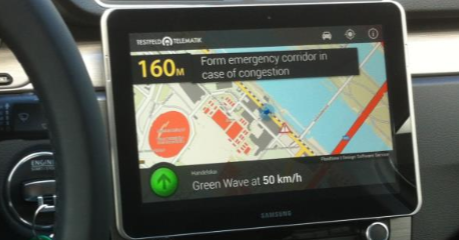
\includegraphics[width=0.7\textwidth]{telematik} 
    \grayRule
    \caption[Projekt Testfeld-Telematik Ampelinformation]{Mobile Anwendung des Projekts Testfeld-Telematik Quelle: \cite{Telematik}}
    \label{fig:telematik}
\end{figure}  
Andere Autohersteller wie BMW, Volvo und Volkswagen kooperieren als Forschungsprojekt "'Car 2 Car Communication Consortium"' mit \textsc{Testfeld Telematik} ebenfalls mit dem Ziel, die Sicherheit an Kreuzungen zu verbessern. Im Auto installierte Sensoren kommunizieren mit Kameras und Scanner in der Ampel. Allerdings funktioniert das System nur, wenn alle Autohersteller zusammenarbeiten und sich auf den gleichen Standard einigen. \cite{Siemens}
\subsection*{Toyota}
Auch Toyota hat ein System entwickelt, welches ebenfalls eine spezielle Infrastruktur an Kreuzungen erfordert (Installation von Infrarot-Sendern, die mit dem Toyota-Navigationssystem kommunizieren). An einer roter Ampel werden die Fahrer über die verbleibende Wartezeit informiert. Die ausgestatteten Navigationssysteme wurden bis jetzt jedoch ausschließlich in Japan getestet. \cite{Toyota}
%
%%% Apps %%% 
%
\subsection{Ampelinformationssysteme als mobile Applikation}
\glspl{Smartphone} sind bereits mit einem \gls{GPS}-Empfänger ausgestattet und haben Internetzugang, was unter anderem die Entwicklung von mobilen Ampelassistenten ermöglicht. Die nachfolgenden Applikationen existieren bereits oder befinden sich in der Testphase.
%%% ENLIGHTEN %%%
\subsection*{Mobile Applikation EnLighten}
Connected Signals ist ein 2014 gegründetes Startup aus Eugene in Oregon (USA), das Echtzeit--Verkehrssignalinformationen sammelt und so Modelle zur Vorhersage von Ampelsignalen entwickelt. Die von Connected Signals erstellte Smartphone Applikation \textsc{EnLighten} bietet Treiber mit Vorhersagen, wie lange man an einer roten Ampel stehen wird. \cite{connectedSignals} \\
Connected Signals verbindet sich mit dem Verkehrsmanagementsystem der jeweiligen Stadt, um Informationen über Signal- und Sensorzustände zu erhalten. Diese Informationen werden sowohl mit der Karte als auch den Geschwindigkeitsbegrenzungen kombiniert und in ein herstellerunabhängiges Format umgewandelt. Connected Signals wendet die proprietäre Technologie an, um den Status der \gls{LSA} abzubilden und eine entsprechende Vorhersage über zukünftiges Verhalten zu treffen. \cite{signals} 
\begin{figure}[t]
    \centering
    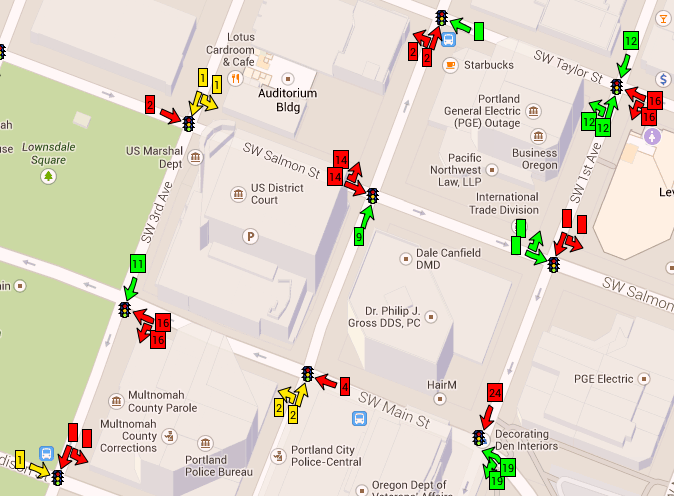
\includegraphics[width=0.7\textwidth]{Portland_live} 
    \grayRule
    \label{fig:enlighten}
    \caption[Connected Signals live Vorhersage]{Live Ampelsignalvorhersage in Portland Quelle: \cite{signals}}
\end{figure}
\textsc{EnLighten} verwendet Informationen über den aktuellen Ampelstatus, Tages- und Stoßzeit und bereits gespeicherte Daten, um eine Vorhersage und dessen Wahrscheinlichkeit zu treffen. Nur bei einer Wahrscheinlichkeit, die hoch genug ist, folglich einer genauen Vorhersage entspricht, visualisiert \textsc{EnLighten} die Restrotdauer. Für eine ungenaue Vorhersage können zum Beispiel Variationen in den Zeitplänen (Stoßzeiten) verantwortlich sein.\\  
Connected Signals nutzt \gls{GPS}, kombiniert mit Auskünften der Fahrzeugsysteme wie den Blinker, Geschwindigkeitsmesser und den Bremspedal-Status zur genauen Lokalisierung des Autos. Um präzise Ampelinformationen zu liefern werden Werkzeuge von der automatischen Erkennung von Lücken in digitalen Stadtplänen, bis hin zur Bestimmung der Ampelphasenpläne und Zeitplänen basierend auf dem Verkehr an Kreuzungen eingesetzt. \cite{EnLighten} \\
\textsc{EnLighten} steht in einer kleinen, aber wachsenden Zahl von Städten in den Vereinigten Staaten zur Verfügung. 
%%% SIGNAL GURU %%%
\subsection*{Mobile Applikation Signal Guru}
Signal Guru wurde von den Wissenschaftlern des MIT\footnote{ Massachusetts Institute of Technology} und der Universität von Princeton entwickelt. Unter den vorgestellten Projekten hebt sich Signal Guru insofern ab, als dass die Informationen nicht direkt von einer Vermittlung (Server oder \gls{LSA}) kommt, sondern von der Anwendung selbst ermittelt wird. Die \Gls{App} errechnet über die \glspl{Smartphone} vieler Nutzer -- welche miteinander kommunizieren -- die Wahrscheinlichkeit, wann eine Ampel grün wird und errechnet daraus ein Zeitmuster zur Vorhersage. Wie in Abbildung \ref{fig:AppSignalGuru} zu sehen ist, muss die eingebaute Kamera durch die Windschutzscheibe die Ampel registrieren. Bei Testläufen im Straßenverkehr vielen die Ergebnise bei statisch geschalteten Ampeln deutlich besser aus als bei angepassten Ampelschaltungen. \cite{SignalGuruPaper}\\ 
\begin{figure}[H]
    \centering
    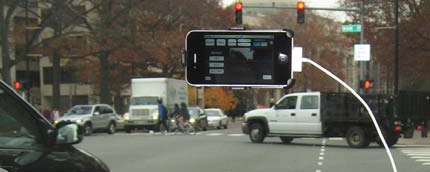
\includegraphics[width=0.7\textwidth]{guru}
    \grayRule
    \caption[Signal Guru]{Signal Guru muss in der Lage sein, die Ampel zu 'sehen'.  Quelle: \cite{SignalGuruPaper}} \label{fig:AppSignalGuru}
\end{figure}
Dieser Ansatz ist für Fahrräder jedoch nicht umsetzbar, da das \gls{Smartphone} in der Halterung am Lenker die \glspl{LSA} nicht erfassen kann.
%
% FAHRRADERWEITERUNGEN %
%
\clearpage
\section{Fahrraderweiterungen}
Um die Fahrräder intelligenter und attraktiver zu machen, gibt es verschiedene Erweiterungen mit zahlreichen Funktionen. Die hier aufgeführten Fahrraderweiterungen führen zum gewünschten Ziel und ergänzen die Navigation um zusätzliche Eigenschaften, die unter anderem den Weg dorthin erleichtern.
\subsection{Displaylose Fahrradnavigation}
Das \textsc{Hammerhead} ist ein Gerät in der Form eines "'Hammers"' und wird an den Fahrradlenker angebracht. Mit verschiedenfarbigen \glspl{LED} bestückt zeigt es den Weg, warnt vor Hindernissen und ersetzt die vorderen Scheinwerfer.\\
Via Bluetooth ist \textsc{Hammerhead} an das \gls{Smartphone} gekoppelt, auf dem die zugehörige Navigationsanwendung läuft mit der man Routen eingeben, teilen und speichern kann. \cite{Hammerhead}\\
\begin{figure}[H]
    \centering
    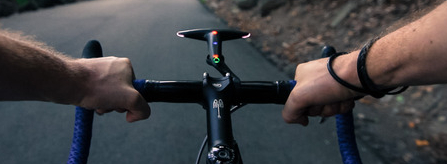
\includegraphics[width=0.7\textwidth]{hammerhead}
    \grayRule
    \caption[Hammerhead]{Hammerhead -- \glspl{LED} zeigen den Weg.  Quelle: \cite{Hammerhead}} 
    \label{fig:hammerhead}
\end{figure}
Ein sehr ähnliches Prinzip verfolgt das \textsc{CycleNav} von der Firma Schwinn. Unterschiede findet man hier im Design und einem integriertem Lautsprecher, der Abbiegehinweise ausgibt und auf Wunsch wiederholt. \cite{CycleNav}
\subsection{Intelligente Fahrradlenker}
Mehr Technologie, aber auch umfangreichere Funktionen bietet der vom amerikanischen Start-up \textsc{Helios-Bikes} entwickelte \textsc{Helios}-Lenker.\\ 
Neben dem Frontlicht hat der Lenker wie in Abbildung \ref{fig:helios} zu sehen, an den Enden \glspl{LED}, die zum gewünschten Ziel leiten. Sie passen ihre Farbe der Geschwindigkeit an und haben auf Wunsch auch eine Blinkfunktion. Verbindet man den Lenker mit einem \gls{Smartphone}, lässt sich die Farbe der \glspl{LED} individualisieren. Die Verbindung zum Handy hat weitere Vorteile: Dank des eingebauten \gls{GPS}-Trackers und eingesteckter SIM-Karte lässt sich das Fahrrad per SMS über den derzeitigen Standort abfragen\cite{Helios}, was im Falle eines Diebstahls sehr hilfreich sein kann.\\ 
\begin{figure}[H]
    \centering
    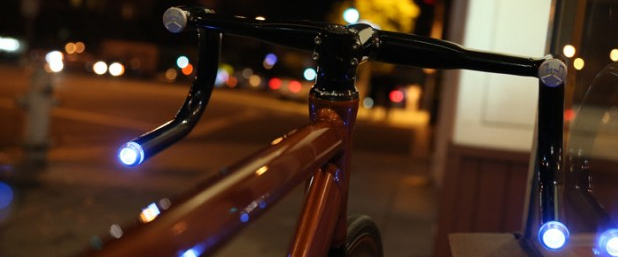
\includegraphics[width=0.7\textwidth]{helios}
    \grayRule
    \caption[Helios-Lenker]{Helios-Lenker  Quelle: \cite{Helios}}		
    \label{fig:helios}
\end{figure}
% ### VANHAWKS ###
\textsc{Vanhawks Valour} heißt das Rad, das ab April 2015 lieferbar ist. Wie im \textsc{Helios}-Lenker steckt auch hier ein über das \gls{Smartphone} steuerbares Navigationssystem, das die Abbiegehinweise per \gls{LED} im Lenker signalisiert. Auf den gefahrenen Routen merkt sich das Rad durch einen Erschütterungssensor erfasste Hindernisse wie Unebenheiten in der Fahrbahn und ermittelt beim nächsten Mal darauf Rücksicht nehmend eine andere Route. Es ist darüber hinaus in der Lage, mit anderen \textsc{Vanhawks valour}-Rädern zu kommunizieren und deren Routenbegebenheiten ebenfalls zu berücksichtigen. Mittels Radarsensoren registriert das Fahrrad Autos im toten Winkel und benachrichtigt die FahrerInnen durch einen vibrierenden Lenker. \cite{vanhawks}
\subsection{Das Samsung Smart Bike}
Auf der Mailänder Designwoche 2014 hatte Samsung ein Smartbike vorgestellt, das mit intelligenten Komponenten wie Bluetooth, einer Kamera und Laserprojektoren ausgestattet ist.\\ 
\begin{figure}[H]
    \centering
    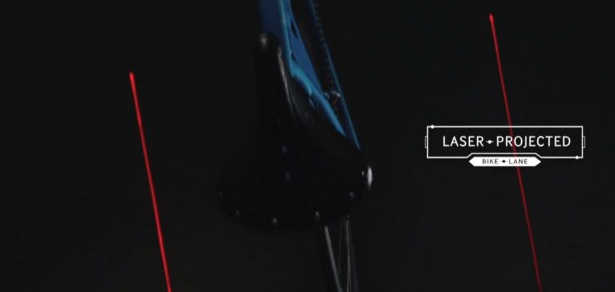
\includegraphics[width=0.7\textwidth]{samsung}
    \grayRule
    \caption[Samsung Smart Bike]{Samsung Smart Bike  Quelle: \cite{smartbike}} 
    \label{fig:samsung}
\end{figure}
Der Rahmen ist aus Aluminium und leicht geschwungen, was Vibrationen abfangen soll.\\
Wie Abbildung \ref{fig:samsung} zeigt, zeichnen vier Laserprojektoren ihren "'eigenen Fahrradweg"' auf die Straße und sollen so die Sicherheit erhöhen, indem sie den Sicherheitsabstand markieren. Natürlich ist auch dieses Fahrrad mit dem \gls{Smartphone} verbunden, das sich dank eines Magneten einfach am Lenker anbringen lässt. Darüber kann man die Laserprojektoren ein- und ausschalten, dafür einen Timer bestimmen und über die eingebaute Kamera unter dem Sattel den Verkehr hinter sich im Auge behalten. Das \gls{Smartphone} fungiert außerdem als Navigationsgerät und durch den eingebauten \gls{GPS} -Empfänger lassen sich eigene und Routen von anderen Nutzern speichern und intelligent verarbeiten. \cite{smartbike}\\ 
Wenn also viele Menschen mit einem Samsung Smartbike auf der gleichen Strecke unterwegs sind, erkennt das Rad die Route als angenehm und navigiert dort entlang.
% ### COBI ###
\subsection{Der COBI Fahrradcomputer}
Ein Projekt aus Frankfurt am Main entwickelt das System \textsc{COBI} (Connected Biking), das alle standardisierten Fahrradsysteme wie Lampen, Navigation, Tachometer etc. vereinen soll. \textsc{COBI} ist ein Modul mit integrierter Frontleuchte, in das man das \gls{Smartphone}, welches dann mit der installierten \textsc{COBI}-\Gls{App} als Fahrradcomputer dient, legt. Durch eine wasser- und stoßfeste Hülle ist es vor Umwelteinflüssen geschützt. Zu dem Lenkersystem gibt es auch Rückstrahler die beim Bremsen intensiver leuchten und eine Blinkfunktion haben.\\
\begin{figure}[H]
        \centering
        \begin{subfigure}[b]{0.49\textwidth}
                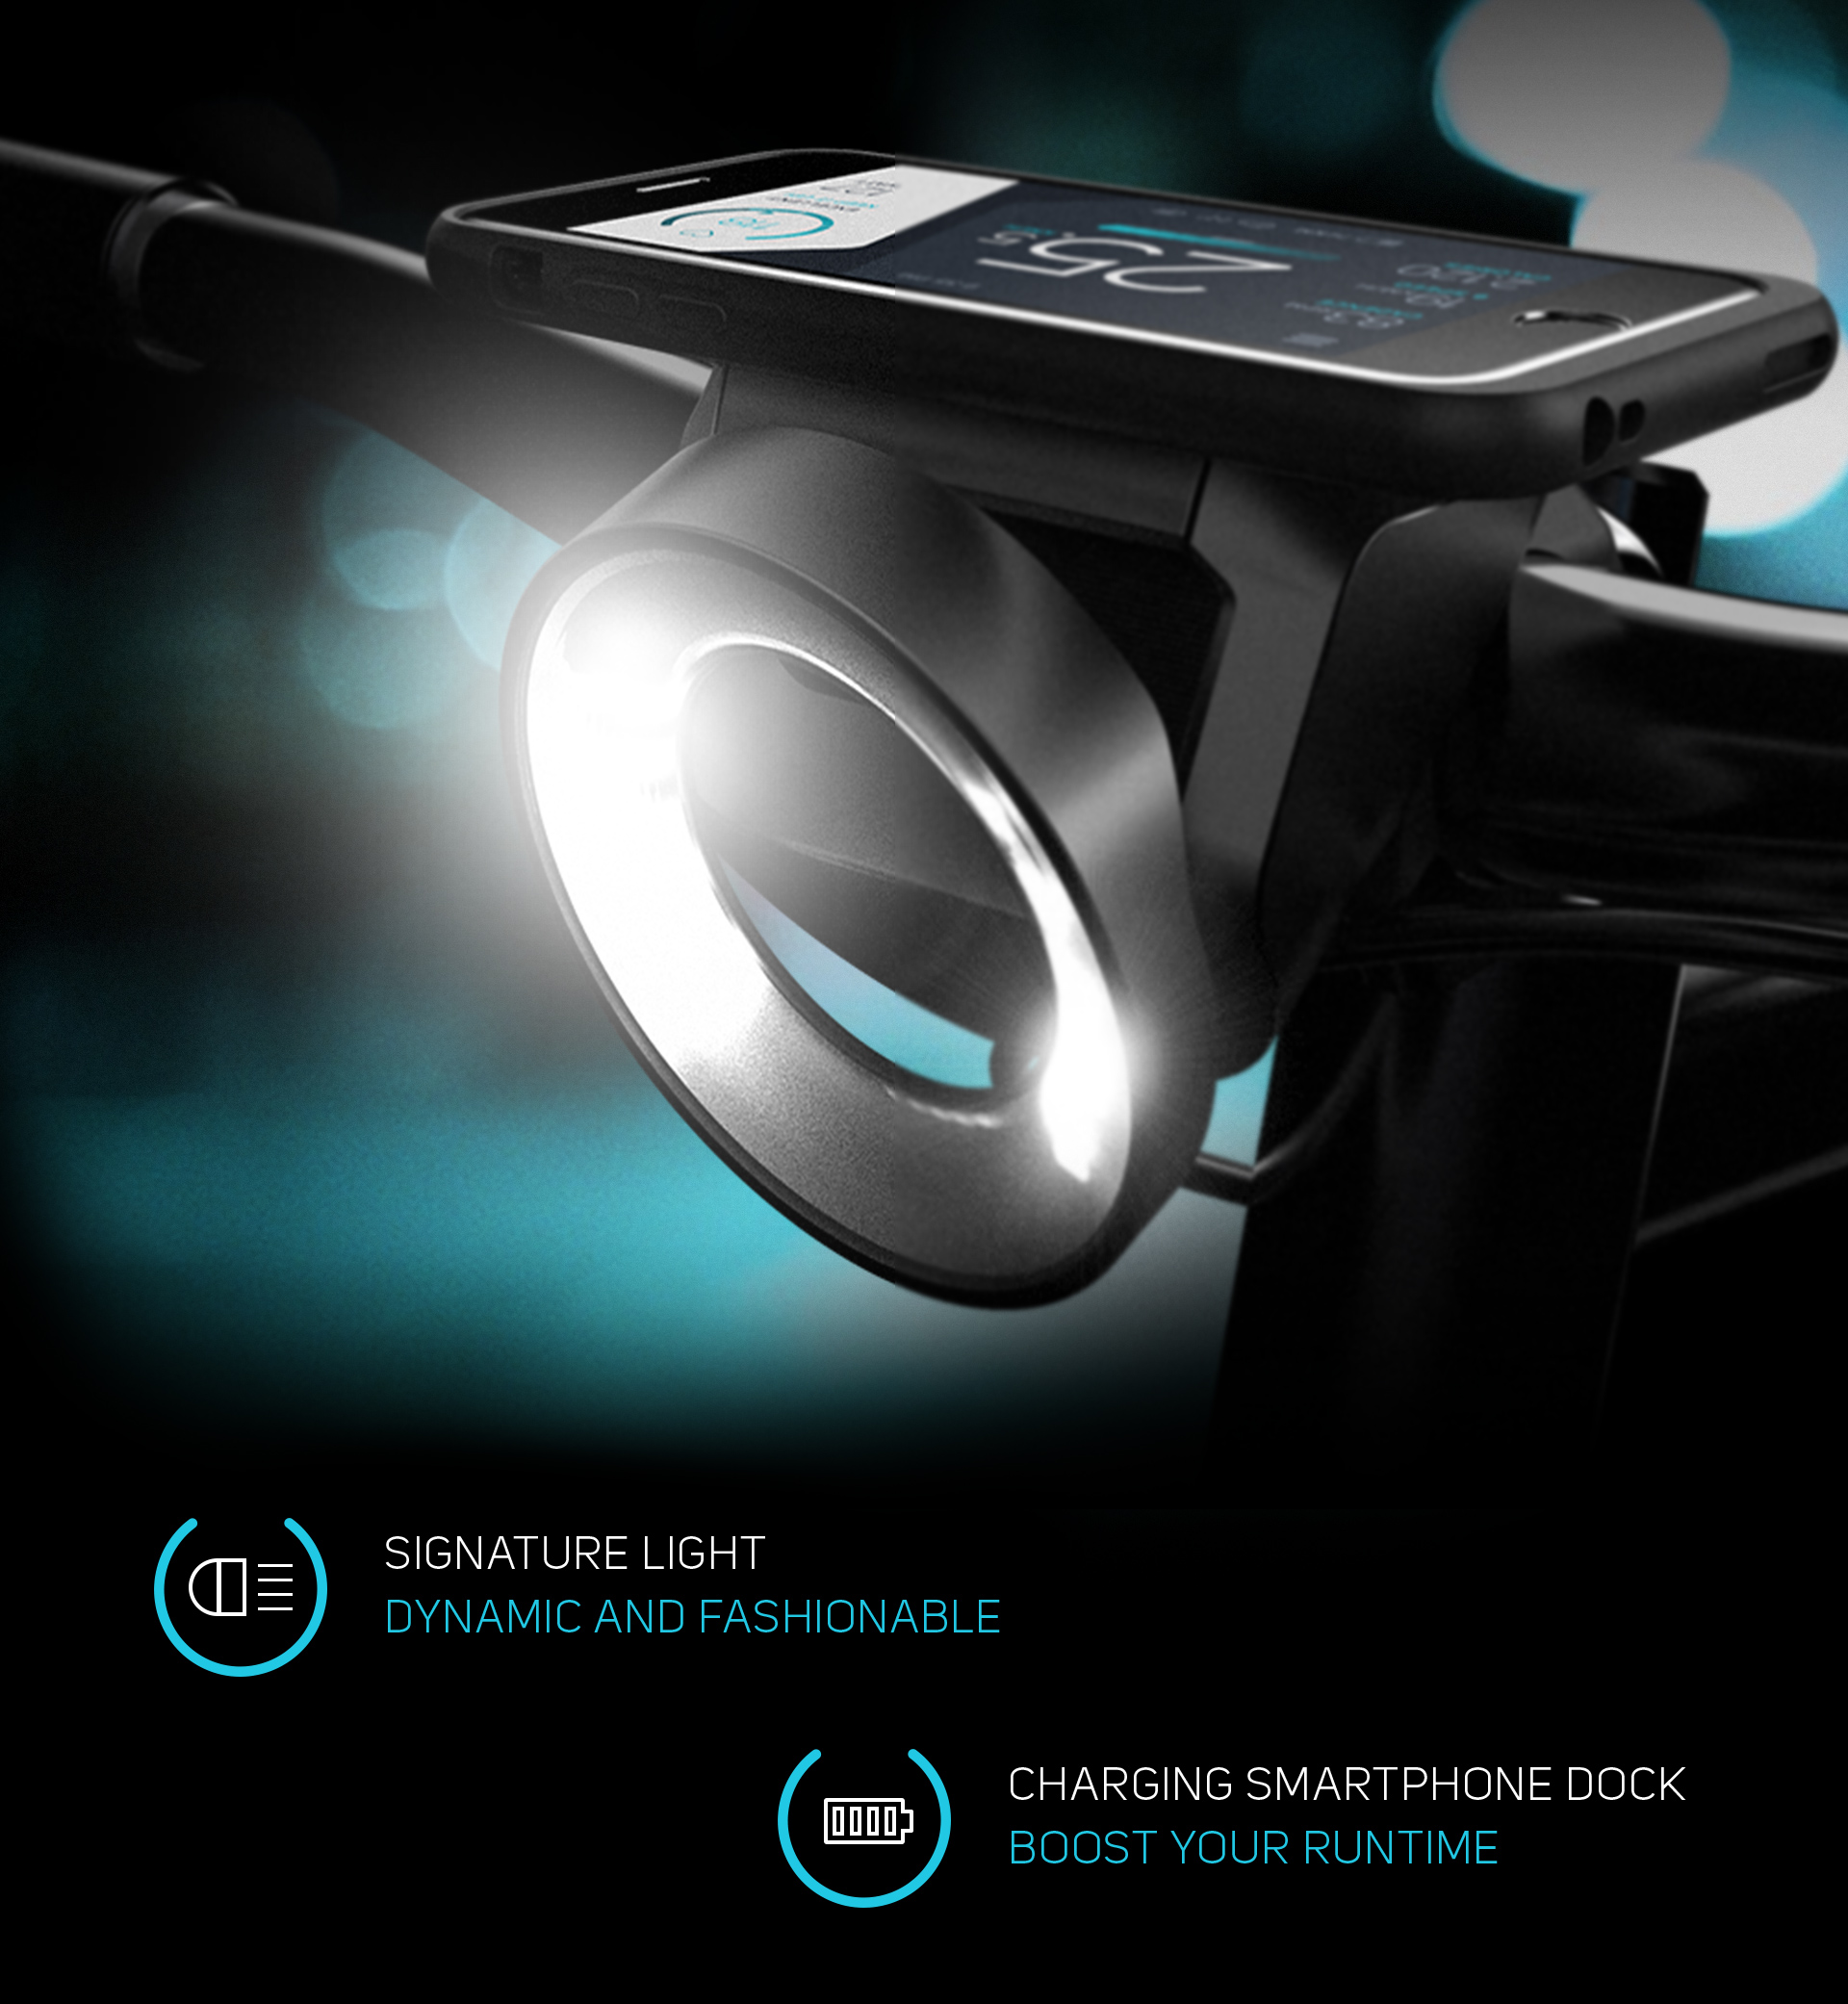
\includegraphics[width=\textwidth]{COBI_01}
                \caption{Frontlicht und Smartphonehalterung}
                \label{fig:cobi1}
        \end{subfigure}%
        ~ %add desired spacing between images (~, \quad, \qquad, \hfill)
        \begin{subfigure}[b]{0.49\textwidth}
                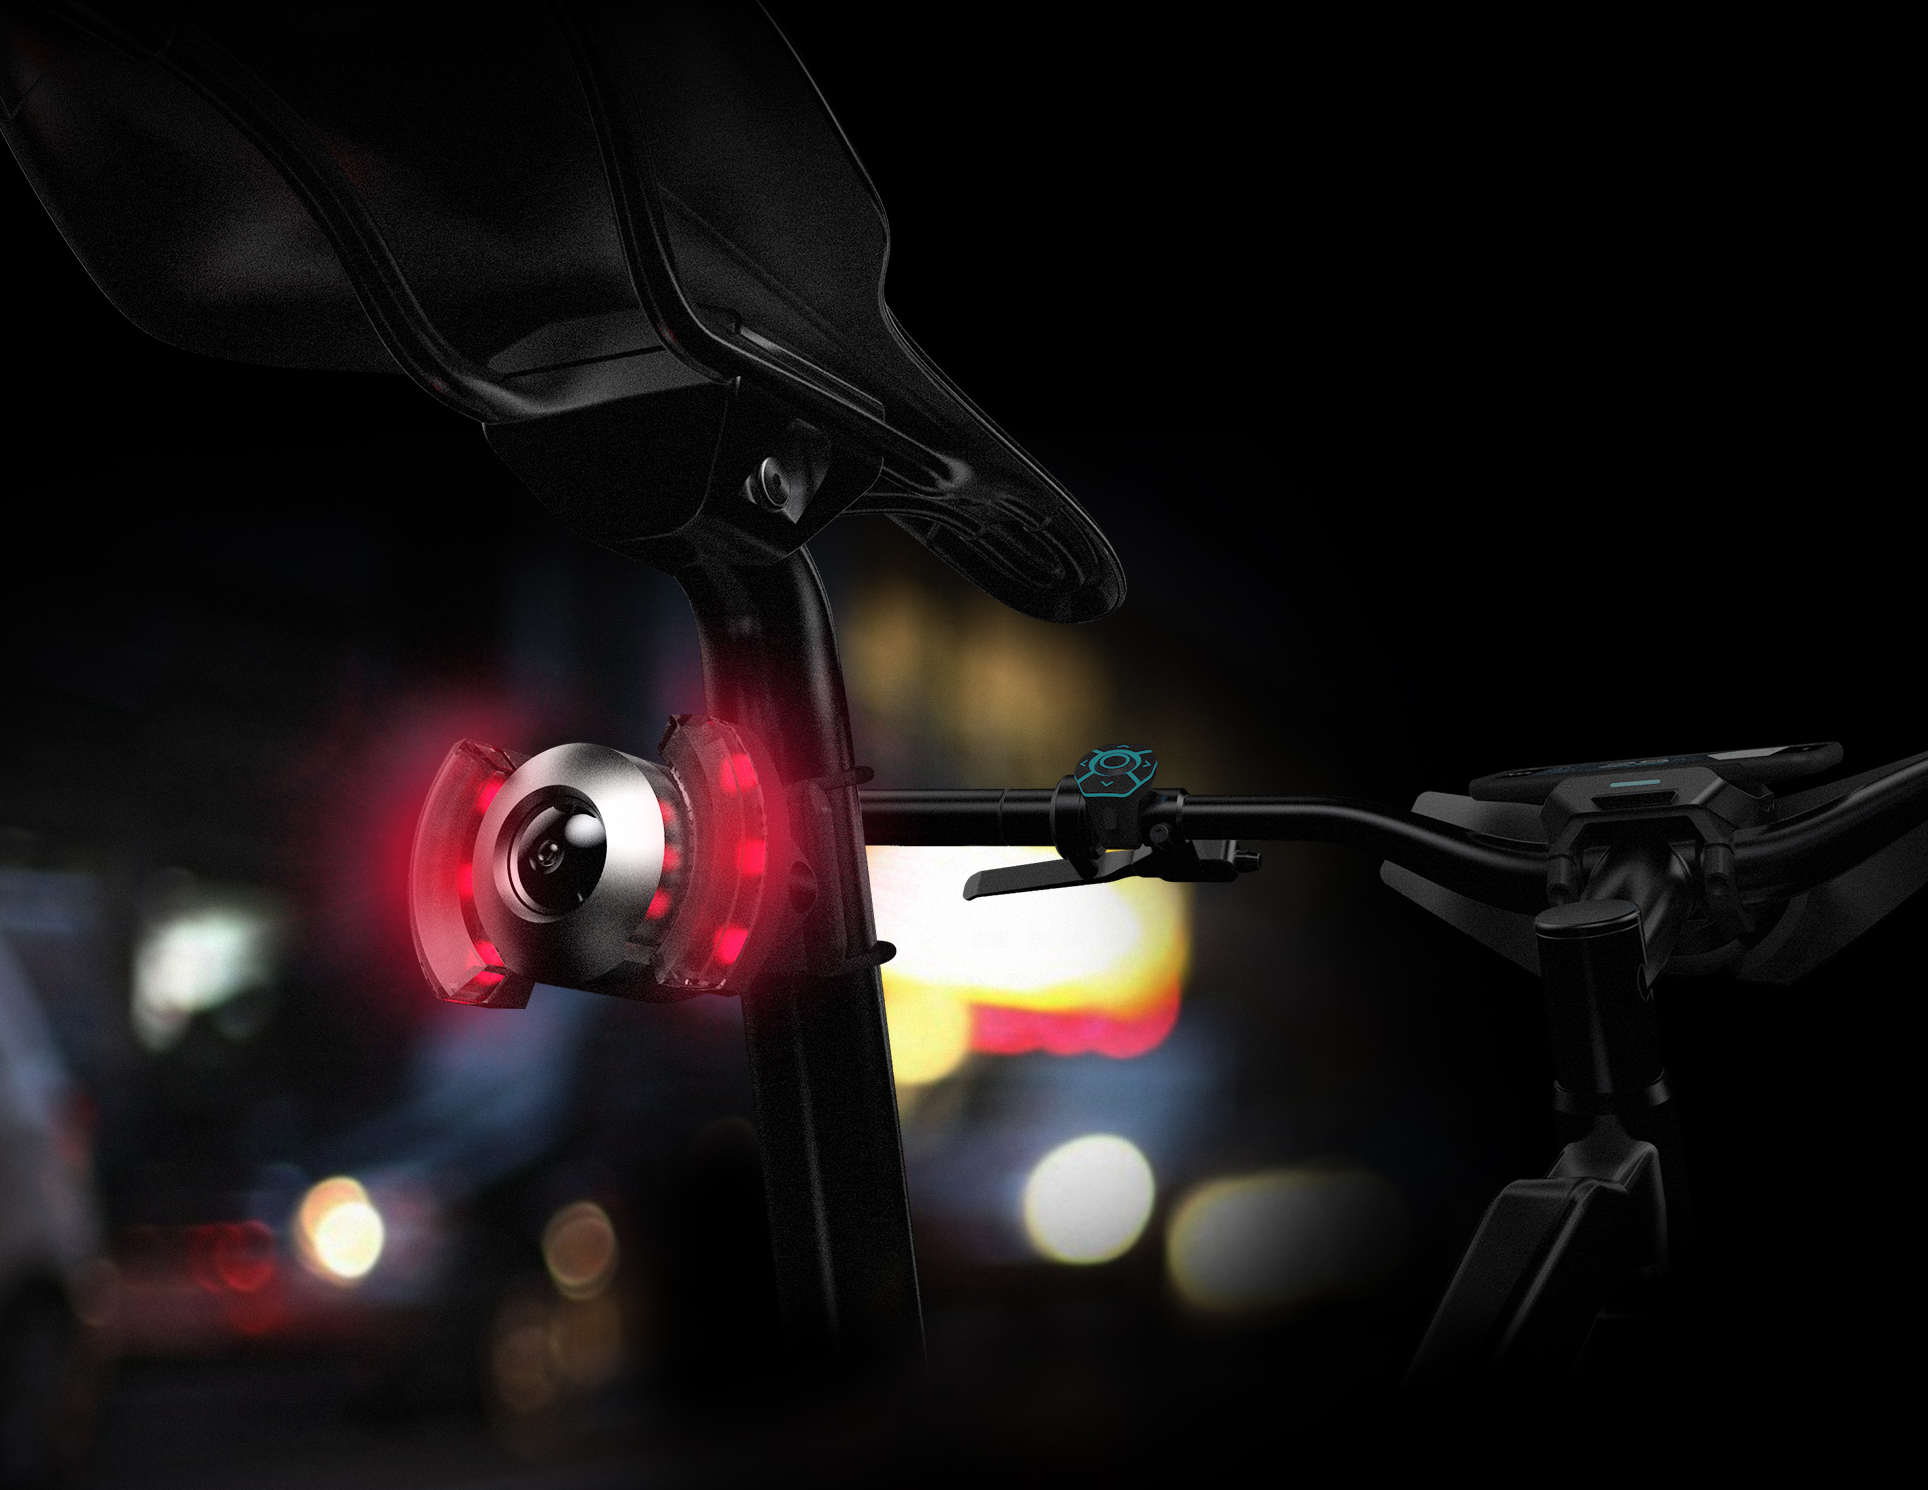
\includegraphics[width=\textwidth]{COBI_02}
                \caption{Bremslicht und Blinker}
                \label{fig:cobi2}
        \end{subfigure}
        \grayRule
        \caption[COBI]{COBI -- Das smarte Fahrradsystem. Quelle: \cite{cobi_pic}}
        \label{fig:cobi}
\end{figure}
Möchte man das \gls{Smartphone} trotzdem nicht am Lenker haben, bleibt die Verbindung zum Modul über Funk bestehen. Steuern lässt sich das System dann über einen Controller, den man am Lenker angebracht, mit dem Daumen bedienen kann. Ist es jedoch in der Halterung, wird das \gls{Smartphone} über den E-Bike-Akku oder einen zusätzlich integrierten Akku aufgeladen. Wie bei den anderen genannten Systemen ist in der \textsc{COBI}-\Gls{App} eine Navigationsanwendung, wie auch die tracking\&share Funktion inklusive. Darüber hinaus verfügt es über einen Diebstahlschutz, Fitnesstracker sowie die Möglichkeit einer Anbindung an Spotify\footnote{ Digitaler Musikstreaming Dienst}.\\
Das Projekt ist bereits voll finanziert und der Versand der vorbestellten Systeme beginnt voraussichtlich im Frühjahr 2015. \cite{cobi}
%%% ERGIBNIS %%%
%\section{Analyseergebnis}
%Das Thema der Geschwindigkeitsempfehlung zum Erreichen der Grünen Welle ist sehr interessant und wird in den nächsten Jahren weiter untersucht werden. Auch die Nachfrage an Fahrraderweiterungen steigt und die EntwicklerInnen solcher Systeme werden kreativer, wodurch immer mehr Produkte mit erweiternden Funktionen entstehen. Es existieren noch andere Studien und Produkte zu diesem Gebiet, doch um den Rahmen dieser Arbeit nicht zu sprengen, werden nicht alle aufgezählt. Sie haben zur Realisierung dieser Arbeit beigetragen indem sie deutlich zeigen, dass sich Forschung zu diesem Thema lohnt.Gerade eine Ampelassistents für das Fahrrad bewegt Menschen dazu, sich für das Radfahren zu begeistern. So wird der Verkehr flüssiger, die Teilnehmer entspannter und die Luft sauberer. AutofahrerInnen sind schon lange nicht mehr allein auf der Straße und so gilt es, dieses erfolgreiche Konzept für alle VerkehrsteilnehmerInnen zu erweitern.
